Now that the requirements necessary to build the system have been formulated, potential solutions to fulfil the list of requirements from Chapter \ref{ch:chapter3} for each aspect of the system can now be analysed before a final solution can be chosen. The first section of this chapter will focus on different solutions for the system's pipeline, starting with the offline feature extraction phase, followed by the online retrieval phase, and ending with the database pre-processing phase. The second section will focus on general design decisions such as the programming language, the type of interface and the type of videos to use. These two sections will be used to conclude with an outline of the final chosen solutions for each aspect of the system.

\section{Pipeline Design Analysis}

In order to chose a global design solution for the system, it is easier to break down the system's pipeline into different phases and review the numerous potential designs for each of these phases. The system pipeline can be split into three different phases, as shown in Figure \ref{fig:basic-cbvr-diagram}:

\begin{itemize}
    \item \textbf{Offline Feature Extraction Phase}. This phase corresponds to the ``training'' phase of the system, where features are extracted from each video in the database and then stored in data files for the retrieval phase.
    \item \textbf{Online Retrieval Phase}. This phase is affiliated to the ``training'' phase of the system, where a single video query is matched to one of the database videos by extracting the same features from the previous phase and comparing them to the stored features.
    \item \textbf{Database Pre-processing Phase}. This is an optional phase where the database videos are processed before the offline feature extraction phase to improve the accuracy and speed of the database videos feature extraction.
\end{itemize}

\begin{figure}[h]
\centerline{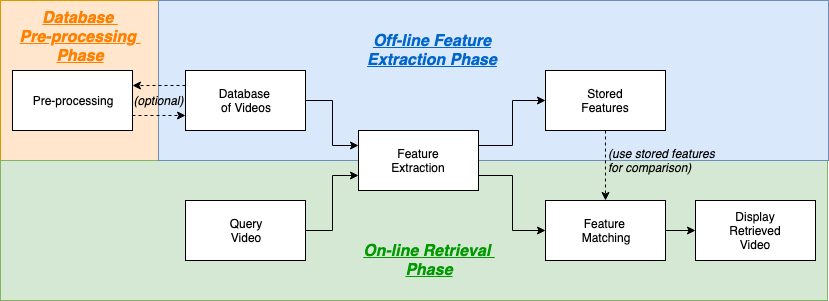
\includegraphics[width=\textwidth]{figures/design/basic_cbvr_phases.png}}
\caption{\label{fig:basic-cbvr-diagram}Basic CBVR system diagram.}
\end{figure}

\begin{comment}
Explore possible options for different sections of the system, such as:
    \begin{itemize}
        \item types of features to extract (why static colour features and not object/motion features) - histograms are very popular with videos, calculations are easier, implementation is easier, results are as efficient
        \item types of learning models (histogram matching, BoW-approach VS Neural Network)
    \end{itemize}
\end{comment}

\subsection{Offline Feature Extraction Phase}
\label{sec:design-offline-feature-extraction}

todo

\subsection{Online Retrieval Phase}
\label{sec:design-online-retrieval}

todo

\subsection{Database Pre-Processing Phase}

todo

\section{General Project Design}

Now that the design choices regarding the system pipeline have been made, general system choices such as the programming language, the interface, the feature storage and the database videos can be inspected.

\subsection{Programming Language}

The programming language is one of the most important aspects when it comes to designing and later implementing the system as it is the medium used to transform the system from design to implementation. However, choosing between 250 different programming languages \cite{tiobe} can be a tricky exercise, which is why multiple views have to be reviewed before a programming language can be chosen. Multiple criteria are considered to justify the choice of the programming languages, including the availability of computer vision-related functions, the runtime speed, the readability and the personal preference.\\

The first element to consider when choosing a programming language for this type of project is the availability of functions for video manipulation and computer vision-related operations. Indeed, using high-level functions to, e.g. read videos or generate histograms is primordial to avoid spending time manually implementing each of these functionalities and to instead devote more time on implementing high-level concepts to complete the pipeline. Some languages such as MATLAB and Python (with mainstream third-party libraries) allow for native manipulation of images/videos and offer collections of computer vision functions. For other programming languages, libraries can be used. The most popular library is OpenCV\footnote{OpenCV, \url{https://opencv.org/}}, which offers functions for real-time computer vision applications. This library supports all the main operating systems (Linux, macOS, Windows, etc.) and although it was mainly designed for C/C++, it contains bindings for the main general-purpose programming languages such as Python, Java, C\#, Javascript, Haskell and MATLAB.\\

Among the previously mentioned programming languages, C/C++ are the fastest languages,
according to \textit{Benchmark Games}\footnote{Benchmark Games: \url{https://benchmarksgame-team.pages.debian.net/benchmarksgame/}}, followed by Java, Javascript and Python, which is considerably slower than the aforementioned programming languages. However, Python can be extended with languages such as C/C++ with ease. This means that coupling Python with the OpenCV library that is initially written in C++ allows the Python code to execute as fast as the original C++ code since it is the actual OpenCV C++ code that is running in the background. Furthermore, Python has an extensive set of third-party libraries that add powerful functionalities to the language, such as Numpy, SciPy and MatplotLib that add mathematical and scientific functions that can compete with MATLAB's native functions. Finally, of all the specified programming languages, Python is the favoured one in terms of personal preference, familiarity, and experience. Therefore, the relatively slower execution speeds of Python that are cancelled out when using OpenCV, coupled with the personal preference for Python, make Python the obvious programming language choice for this project.\\

TODO: add table of pros and cons in appendix

\subsection{Query Video}

pre-recorded, manually crop

\subsection{Interface}

Now that is has been decided that Python will be the programming language used to implement the system, the next decision is the type of interface that will be used to present the results. Although it was specified in Chapter \ref{ch:chapter1} that the system is meant to target mobile devices, creating a mobile application is a waste of time and resources for a project with such a narrow time frame. Despite the fact that Python offers many choices of creating native GUIs using frameworks such as Tkinter, PyQt or WxPython, or simply creating HTML websites, building a graphical interface would take as much time as developing the entire system pipeline. Indeed, the main goal is to complete the different phases of pipeline that will process and match a query video to a database video. Spending time on designing a GUI\footnote{Graphical User Interface} for a mobile device is unnecessary as the objective is not to create a commercial application that can be tested with users, but to develop the matching algorithm that would work in the background of such an application.\\

The only pieces of information that need to be displayed are the following:
\begin{itemize}
    \item Progress of current phase e.g. during the offline feature extraction phase, specify how many videos have been processed and how many are left.
    \item Histograms: display the generated histograms for each video.
    \item Manual Cropping: display the video have have the user manually select the region of interest.
    \item Results:
    \begin{itemize}
        \item The distance measurements between the query video and each database videos, while specifying which distance metric is used.
        \item The final result, which should correspond to a thumbnail of the matched video.
        \item Additional data to measure the efficiency e.g. the runtime and the accuracy (comparison of the number of true positives and the number of false positives)
    \end{itemize}
\end{itemize}

Most of the information previously mentioned can be displayed directly in the console, such as the current phase progress, the distance measurements and the efficiency results. The only graphical requirements is for the manual query cropping, the histograms and the final result output. The OpenCV GUI functions can be used to display the video in a new window and to manually draw the contour of the region of interest as automatically detecting the edges of the screen in the query video would is a very complex task on its own. Regarding the histograms and the final result, it is important to show visual representations of the histograms and the matched video as it was noticed that during the demonstration of progress in February, simply printing the title of the matched video did not provide a sense of accomplishment. Therefore, displaying the histograms and the matched video result can be done through MatplotLib, which is a library used to display plots (histograms) and images (thumbnail of the matched video).

\subsection{Feature Storing File Type}

The features extracted during the offline feature extraction phase (see Section \ref{sec:design-offline-feature-extraction}) and used during the online retrieval phase (see Section \ref{sec:design-online-retrieval}) can either be stored in text files or binary files. Due to the small amount of spread data (three histograms for each video) and the advantages of being able to view the data being written to the text files for debugging purposes, plain text files are the chosen file types for storing the features extracted from the database videos. For a complete list of pros and cons between text files and binary files, see Appendix \ref{ch:appendix-comparison-text-vs-binary}.

\subsection{Database videos}

types of videos in databases (why short videos VS movies, cartoons/stop-motion pictures)

\section{Chosen Solution}

\begin{enumerate}
    \item \textbf{Programming Language}: Python
    \item \textbf{Query Video}: Manual crop
    \item \textbf{Interface}: mainly command line for printing data, along with OpenCV GUI for the query video cropping and MatplotLib for displaying the histograms and results.
    \item \textbf{Feature Storing File Type}: Plain Text files.
\end{enumerate}

\section{Summary}

summarise section
